\chapter{Meilenstein III}
\label{cha:ms3}

Nachdem die vorangegangenen Teilschritte eine Einleitung in die verwendete Technologie dargestellt haben, konstituiert der dritte Meilenstein den ersten Abschnitt des gruppenspezifischen Projektes. Ziel ist es eine eigene Anwendung zu konzipieren, Hard/Software-Anforderungen zu ermitteln und ein Grundgerüst zu implementieren und zu testen.


\section{Smart Mirror}

\begin{figure}
	\centering
	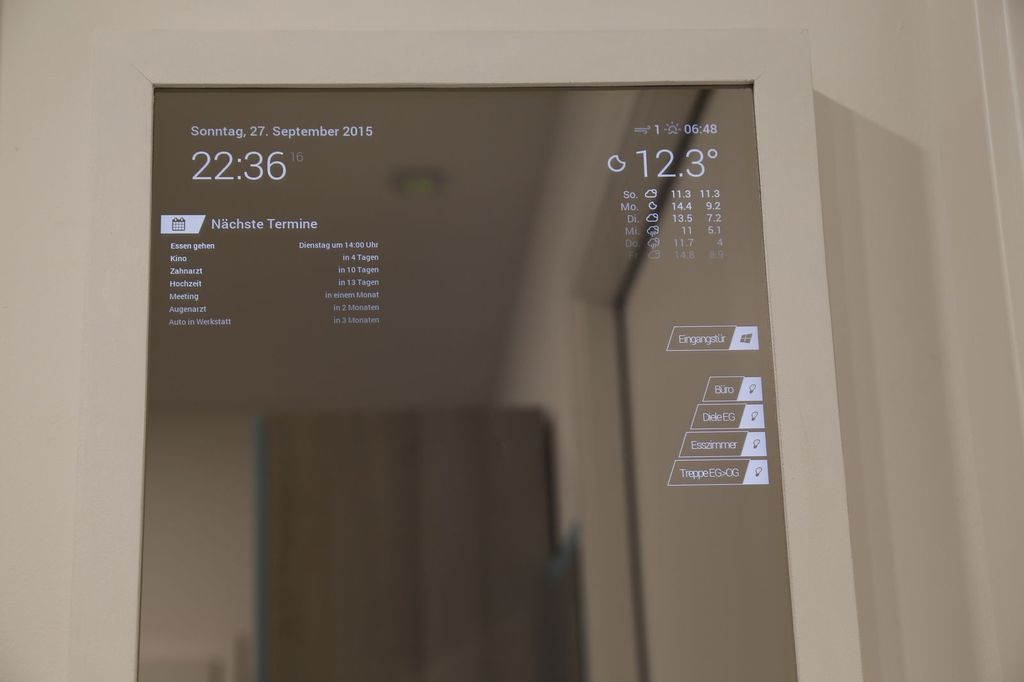
\includegraphics[width=1\textwidth]{figures/sm.JPG}
	\caption{Darstellung Smart Mirror}
	\addloflink{https://community.openhab.org/t/smart-mirror-and-openhab/3611/3}
	\label{img:imirror}
\end{figure}

Wie in Abbildung \ref{img:imirror} dargestellt wird ist der intelligente Spiegel eine Form von erweiterter Realität. Die grundlegende Funktionalität wird ergänzt durch die Darstellung digitaler Informationen wie Kalendereinträgen, Wetterdaten oder aktueller Nachrichten. Aufbauend auf diesem Konzept haben wir uns entschieden eine Nutzeridentifikation durch Gesichtserkennung hinzuzufügen. Die Idee dahinter ist, die dargestellten Daten den Bedürfnissen und Vorlieben des jeweiligen Anwenders anzupassen. 

\begin{table}[]
\centering
\caption{Struktur Smart Mirror}
\label{my-label}
\begin{tabular}{@{}|l|l|@{}}
\toprule
Teilsystem                         & Komponente       \\ \midrule
\multirow{3}{*}{Gesichtserkennung} & OpenCV           \\ \cmidrule(l){2-2} 
                                   & OpenFace         \\ \cmidrule(l){2-2} 
                                   & Camera Module v2 \\ \midrule
\multirow{3}{*}{Informationen}     & Calendar API     \\ \cmidrule(l){2-2} 
                                   & Wetter API       \\ \cmidrule(l){2-2} 
                                   & RSS Feed         \\ \midrule
Darstellung                        & JavaFX           \\ \bottomrule
\end{tabular}
\label{tab:smirror}
\end{table}

Für die Umsetzung des Projektes haben wir uns entschieden Gesichtserkennung und Informationsservices auf separaten Plattformen zu implementieren. Es wird ein Raspberry Pi verwendet um die Gesichtserkennung durchzuführen und darauffolgend die Nutzeridentifikation an den SSP zu senden. Ein weiterer Pi wird zur Informationsbeschaffung sowie Darstellung auf dem display genutzt. Dazu werden die Nutzerdaten am SSP abgefragt und die zugeordneten Datensätze heruntergeladen. 

Tabelle \ref{tab:smirror} zeigt die Gliederung des Smart Mirror in Teilsysteme deren Komponenten bereits in Kapitel \ref{cha:config} vorgestellt wurden. Im Folgenden wird die Implementierung der einzelnen Teilsysteme vorgestellt.


\subsection{Gesichtserkennung}
\label{subsec:facedetection}

Um unterschiedliche Benutzer mithilfe einer Kamera zu erkennen wird eine Gesichtserkennung benötigt. Dazu wird das Python Paket face\_recognition\footnote{https://pypi.python.org/pypi/face\_recognition}\footnote{https://github.com/ageitgey/face\_recognition} genutzt, welches selbst wiederum auf der Bibliothek dlib aufbaut, um die Gesichtserkennung zu ermöglichen. Mithilfe des Pakets face\_recognition ist es mit wenigen Codezeilen möglich eine sehr robuste Gesichtserkennung zur Verfügung zu stellen. Ein solches Python Skript findet sich in \ref{code:pythonFaceRec} . Um das Paket face\_recognition auf einem RaspberryPi verwenden zu können müssen mehrere weitere Pakete, sowie die dlib Bibliothek installiert werden. Im Git des face\_recognition Projekts findet sich dazu eine ausführliche Anleitung\footnote{https://gist.github.com/ageitgey/1ac8dbe8572f3f533df6269dab35df65}.
Zusätzlich wurde Bibliothek OpenCV verwendet. Dies ist nicht zwingend für die Gesichtserkennung notwendig, vereinfacht jedoch die Handhabung der Bilder.
EIne Anleitung zur Installation von OpenCV 3 findet sich unter \footnote{http://www.pyimagesearch.com/2016/04/18/install-guide-raspberry-pi-3-raspbian-jessie-opencv-3/} .

Anschließend an die Installation kann die Gesichtserkennung mit dem gegebenen Python Skript aus \ref{code:pythonFaceRec} erfolgen. Um die vom Skript erkannten und ausgegebenen Gesichter in den SSP eintragen zu können, wird das Skript von einem Java Programm gestartet. Ein Code Beispiel dazu ist in \ref{code:javaFaceRec} zu finden. Die eingelesenen Namen können auf die gleiche Art wie ursprünglich die Lux werte in den SSP eingetragen werden.

Die Qualität der Gesichtserkennung ist bei dem von uns verwendeten Verfahren extrem robust. Es reicht ein einziges Referenzbild von jeder zu erkennenden Person um diese aus fast allen Winkeln zu erkennen. Auch die Geschwindigkeit ist ausreichend. Es dauert höchstens 1-2 Sekunden um eine sich vor der Kamera befindende Person zu erkennen. Die Geschwindigkeit sinkt dabei mit steigender Anzahl von Personen vor der Kamera. 


\begin{lstlisting}[language=Python,caption={Python Skript für Gesichtserkennung mithilfe von face\_recognition},label=code:pythonFaceRec]
import face_recognition
import cv2
import time
from picamera.array import PiRGBArray
from picamera import PiCamera

# initialize the camera and grab a reference to the raw camera capture
camera = PiCamera()
camera.resolution = (1280, 960)
camera.framerate = 32
rawCapture = PiRGBArray(camera, size=(1280, 960))
time.sleep(1)

# Load a sample picture and learn how to recognize it.
person1_image = face_recognition.load_image_file("/home/pi/face_recognition/examples/person1.jpg")
person2_image = face_recognition.load_image_file("/home/pi/face_recognition/examples/person2.jpg")
person1_face_encoding = face_recognition.face_encodings(dominik_image)[0]
person2_face_encoding = face_recognition.face_encodings(biden_image)[0]

# Initialize some variables
face_locations = []
face_encodings = []
face_names = []
scale = 8

for frame in camera.capture_continuous(rawCapture, format="bgr", use_video_port=True):
	# Grab a single frame of video
	frame = frame.array

	# Resize frame of video to 1/4 size for faster face recognition processing
	small_frame = cv2.resize(frame, (0, 0), fx=(1/scale), fy=(1/scale))

	# Find all the faces and face encodings in the current frame of video
	face_locations = face_recognition.face_locations(small_frame)
	face_encodings = face_recognition.face_encodings(small_frame, face_locations)

	face_names = []
	for face_encoding in face_encodings:
		# See if the face is a match for the known face(s)
		match = face_recognition.compare_faces([person1_face_encoding,person2_face_encoding], face_encoding)
		name = "Unknown"

		if match[0]:
			name = "Person1"
		if match[1]:
			name = "Person2"
		print(name)
		face_names.append(name)

# Release handle to the webcam
video_capture.release()
cv2.destroyAllWindows()
\end{lstlisting} 

\begin{lstlisting}[language=Python,float=htb,caption={Java Code zum starten und auslesen des Python Scripts},label=code:javaFaceRec]
public void run() {
try {
System.out.println("Start FaceRec");
ProcessBuilder pb = new ProcessBuilder("python","-u", "/home/pi/face_recognition/facerec.py");
pb.redirectOutput(Redirect.PIPE);
Process p = pb.start();
BufferedReader reader = new BufferedReader(new InputStreamReader(p.getInputStream()));
String line = null;

while (true) {
try {
p.exitValue();
break;
} catch (Exception e) {
}
while ((line = reader.readLine()) != null) {
faceRecService.setName(line);
}
}
System.out.println("Stop FaceRec");
} catch (IOException e) {
e.printStackTrace();
}
}
\end{lstlisting}

\begin{figure}
	\centering
	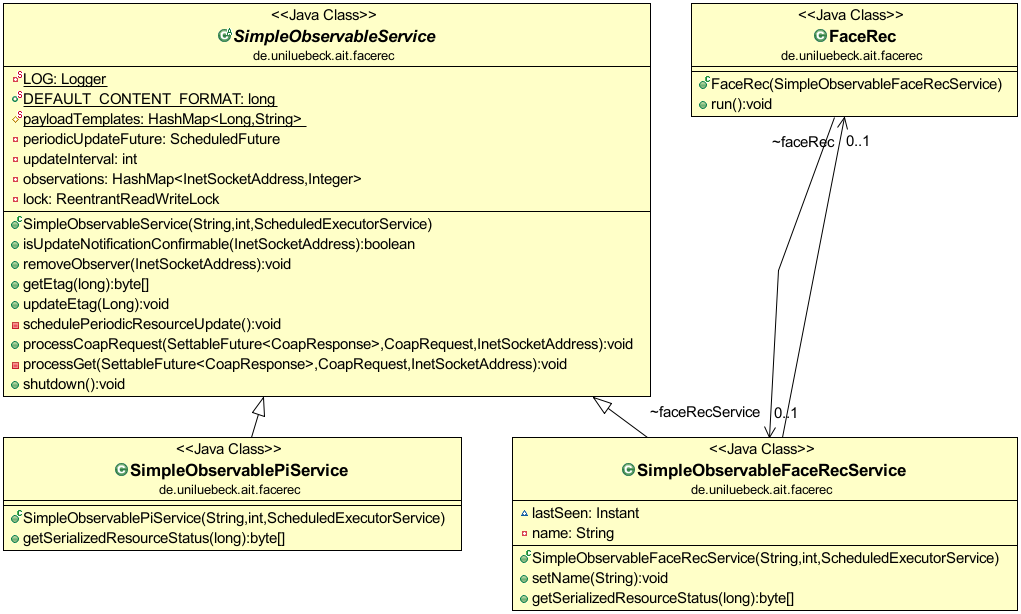
\includegraphics[width=1\textwidth]{figures/facerecservice.png}
	\caption{Klassendiagramm des Observable Service für die Gesichtserkennung}
	\label{img:facerec}
\end{figure}


\subsection{Informationen}
\label{subsec:information}

Die auf dem Spiegel dargestellten Informationen umfassen aktuelles Wetter sowie eine Vorhersage für die nächsten Tage und benutzerspezifische Informationen in form von Kalendereinträgen und präferierten Nachrichtenfeeds. In Abbildung \ref{img:infoclasses} werden die entsprechenden Services und deren Aggregation in der für die Darstellung zuständigen Klassen beschrieben.

\begin{figure}
	\centering
	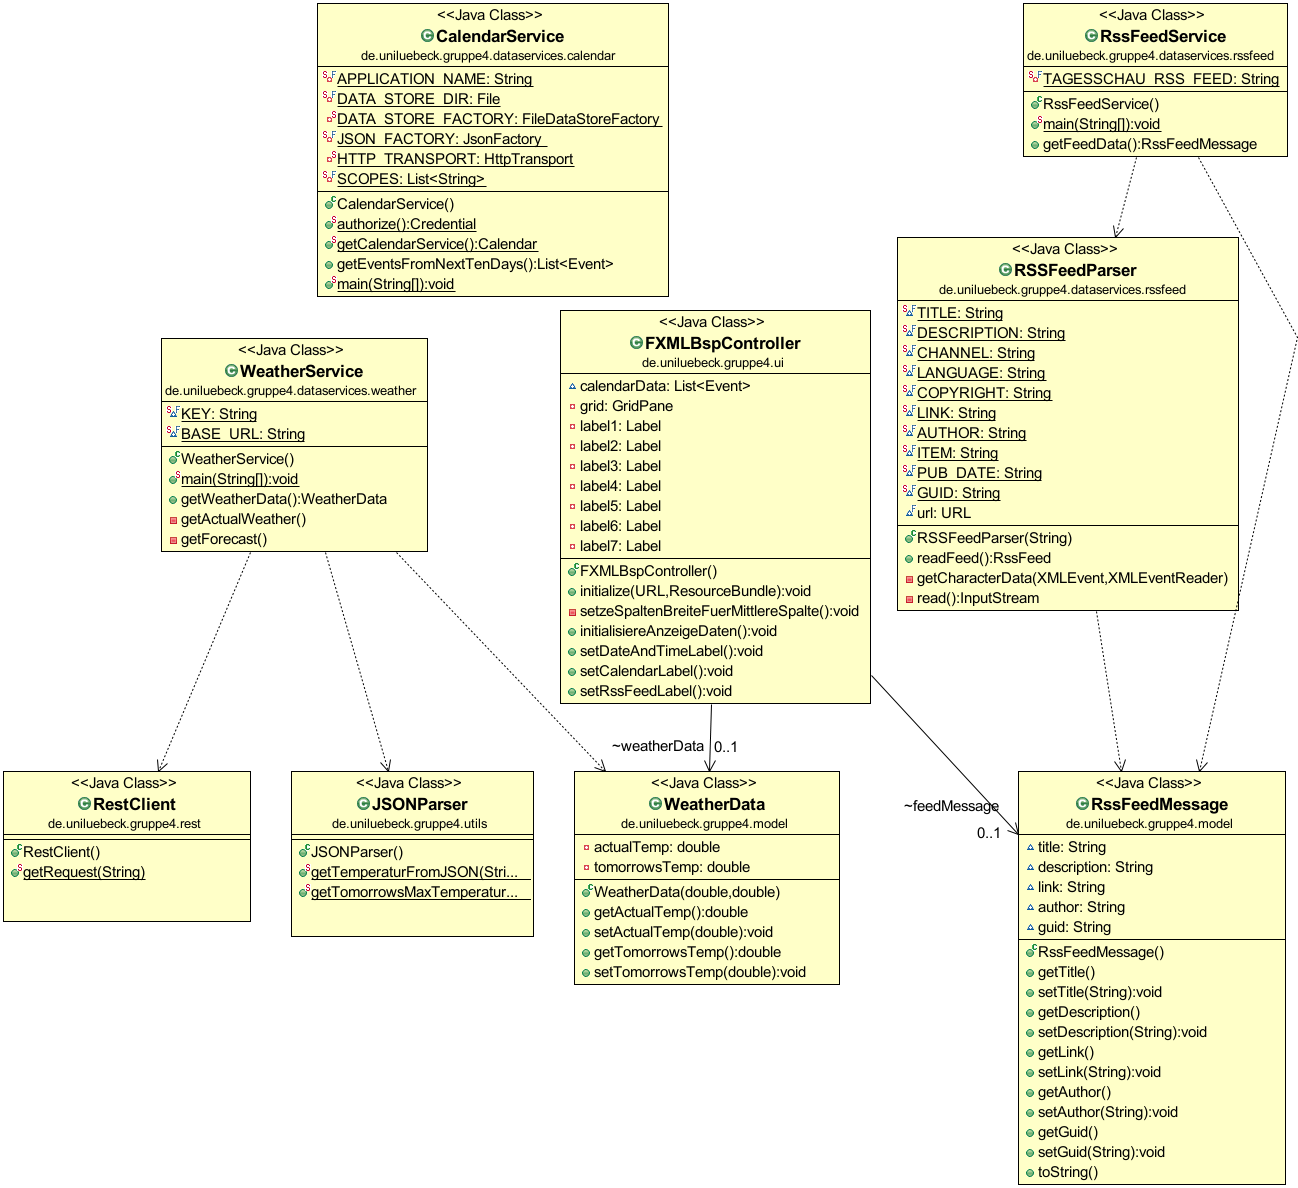
\includegraphics[width=1\textwidth]{figures/infoclasses.png}
	\caption{Klassendiagramm der Informationsservices mit Bezug auf die Darstellung im Display}
	\label{img:infoclasses}
\end{figure}

\subsubsection{Nachrichten}
\label{subsubsec:news}

Wie in Abschnitt \ref{subsubsec:rss} beschrieben ist es möglich mittels RSS-Feeds automatisiert Aktualisierungen auf Websites zu verfolgen. In dieser Anwendung wird die Technologie benutzt um eine dem Nutzer zugeordnete Nachrichtenquelle abzurufen und die Informationen auf dem Display darzustellen. Die gewünschten Informationen werden in einer XML-Datei heruntergeladen und, wie in Abbildung \ref{code:readFeed} dargestellt, unter Benutzung des \textit{javax.xml package} in die für die Darstellung relevanten Blöcke zerlegt.

\begin{lstlisting}[float=htb,caption={RRSFeedParser Klasse - Auslesen der Informationen aus empfangenem XML Dokument},label=code:readFeed]
	// First create a new XMLInputFactory
   	XMLInputFactory inputFactory = XMLInputFactory.newInstance();
    // Setup a new eventReader
    InputStream in = read();
    XMLEventReader eventReader = inputFactory.createXMLEventReader(in);
    // read the XML document
    while (eventReader.hasNext()) {
    	XMLEvent event = eventReader.nextEvent();
        if (event.isStartElement()) {
        String localPart = event.asStartElement().getName().getLocalPart();
        	switch (localPart) {
                case ITEM:
            	if (isFeedHeader) {
                 	isFeedHeader = false;
                       	feed = new RssFeed(title, link, description, language,
                                    copyright, pubdate);
                  	}
                    event = eventReader.nextEvent();
                    break;
                		...
            	}
           	} else if (event.isEndElement()) {
            	if (event.asEndElement().getName().getLocalPart() == (ITEM)) {
                    RssFeedMessage message = new RssFeedMessage();
                    message.setAuthor(author);
                    message.setDescription(description);
                    message.setGuid(guid);
                    message.setLink(link);
                    message.setTitle(title);
                    feed.getMessages().add(message);
                    event = eventReader.nextEvent();
                	continue;
            	}
            }
        }
    } catch (XMLStreamException e) {
		throw new RuntimeException(e);
    }
    return feed;
}
\end{lstlisting}

\subsubsection{Wetter}
\label{subsubsec:weather}

Nach erfolgreicher Registrierung bei dem Dienstleister Openweathermap \footnote{\url{openweathermap.org}, Abschnitt \ref{subsubsec:weather}} wird ein Schlüssel bereitgestellt, welcher einen Zugriff auf deren API ermöglicht. Darüber können die benötigten lokalen Wetterdaten in Form einer \textit{*.json} kostenfrei bezogen werden. In Codeabschnitt \ref{code:weather} werden sowohl der Request als auch die Zerlegung in relevante Blöcke, mittels \textit{JSONParser} beschrieben.

\begin{lstlisting}[float=htb,caption={WeatherService Klasse zum Abrufen der aktuellen Wetterlage sowie Vorhersage für eine Region},label=code:weather]
package de.uniluebeck.gruppe4.dataservices.weather;

import de.uniluebeck.gruppe4.model.WeatherData;
import de.uniluebeck.gruppe4.rest.RestClient;
import de.uniluebeck.gruppe4.utils.JSONParser;

public class WeatherService {

	static final String KEY = "appid=da7c4d55907d8cff81b1e5a02bae88e6";
	static final String BASE_URL = "http://api.openweathermap.org/data/2.5/";
	
	public static void main(String[] args) {
		WeatherService service = new WeatherService();
		WeatherData data = service.getWeatherData();
	}
	
	public WeatherData getWeatherData(){
		String actualWeather = getActualWeather();
		String forecast = getForecast();
		
		double actualTemp = JSONParser.getTemperaturFromJSON(actualWeather);
		double tomorrowTemp = JSONParser.getTomorrowsMaxTemperaturFromJSON(forecast);
		
		WeatherData weatherData = new WeatherData(actualTemp, tomorrowTemp);
		
		return weatherData;
	}
	
	private String getActualWeather() {
		return RestClient.getRequest(BASE_URL + "weather?q=London,uk&" + KEY);
	}
	
	private String getForecast(){
		return RestClient.getRequest(BASE_URL + "forecast?q=London,uk&" + KEY);
	}
}
\end{lstlisting}


\subsubsection{Kalender}
\label{subsubsec:calendar}

Um die Darstellung der Kalenderinformationen zu implementieren haben wir uns entschieden die entsprechende Google-API \footnote{\url{https://developers.google.com/google-apps/calendar/}} zu nutzen. In diesem Rahmen wurde ein Benutzerkonto für \textit{Max Mustermann} angelegt. Der Zugriff auf die entsprechenden daten erfordert die Erstellung eines \textit{Credential Objects}, der Vorgang ist in Codeabschnitt \ref{code:calendar} dargestellt.

\begin{lstlisting}[float=htb,caption={CalendarService Klasse - Authorisierung des jeweiligen Anwenders},label=code:calendar]
    /**
     * Creates an authorized Credential object.
     * @return an authorized Credential object.
     * @throws IOException
     */
    public static Credential authorize() throws IOException {
        // Load client secrets.
        InputStream in =
            CalendarService.class.getResourceAsStream("/client_secret.json");
        GoogleClientSecrets clientSecrets =
            GoogleClientSecrets.load(JSON_FACTORY, new InputStreamReader(in));

        // Build flow and trigger user authorization request.
        GoogleAuthorizationCodeFlow flow =
                new GoogleAuthorizationCodeFlow.Builder(
                        HTTP_TRANSPORT, JSON_FACTORY, clientSecrets, SCOPES)
                .setDataStoreFactory(DATA_STORE_FACTORY)
                .setAccessType("offline")
                .build();
	// Credential credential = new AuthorizationCodeInstalledApp(
	// flow, new LocalServerReceiver()).authorize("user");

        Credential credential = new AuthorizationCodeInstalledApp(
                flow, new LocalServerReceiver()).authorize("Max_Mustermann");
        
        System.out.println(
                "Credentials saved to " + DATA_STORE_DIR.getAbsolutePath());
        return credential;
    }
\end{lstlisting}


\subsection{Darstellung}
\label{subsec:display}

Die UI befindet sich noch in der Entwicklung. Sie wird mittels JavaFx realisiert. Den aktuellen Stand zeigt Figure \ref{img:mirror_ui}, anhand derer man sich eine grobe Vorstellung holen kann, wie das Ganze aufgebaut ist. Aktuell sind 3 Anzeige-Flächen für Informationen geplant: Die linke Spalte, für das aktuelle Datum, die Uhrzeit und anstehende Termine aus dem Google-Kalendar, die rechte Spalte für Wetter-Informationen und eine Fußzeile mit einem Auszug der aktuellsten Nachrichten. In der Mitte wird dann platz gelassen für das Spiegelbild.
Hierzu wurde als Layout-Element von JavaFx der BorderPane gewählt, welcher bereits in diese Left, Right, Top, Bottom und Center Regionen aufgeteilt ist (siehe Figure \ref{img:mirror_borderpane}).


\begin{figure}
	\centering
	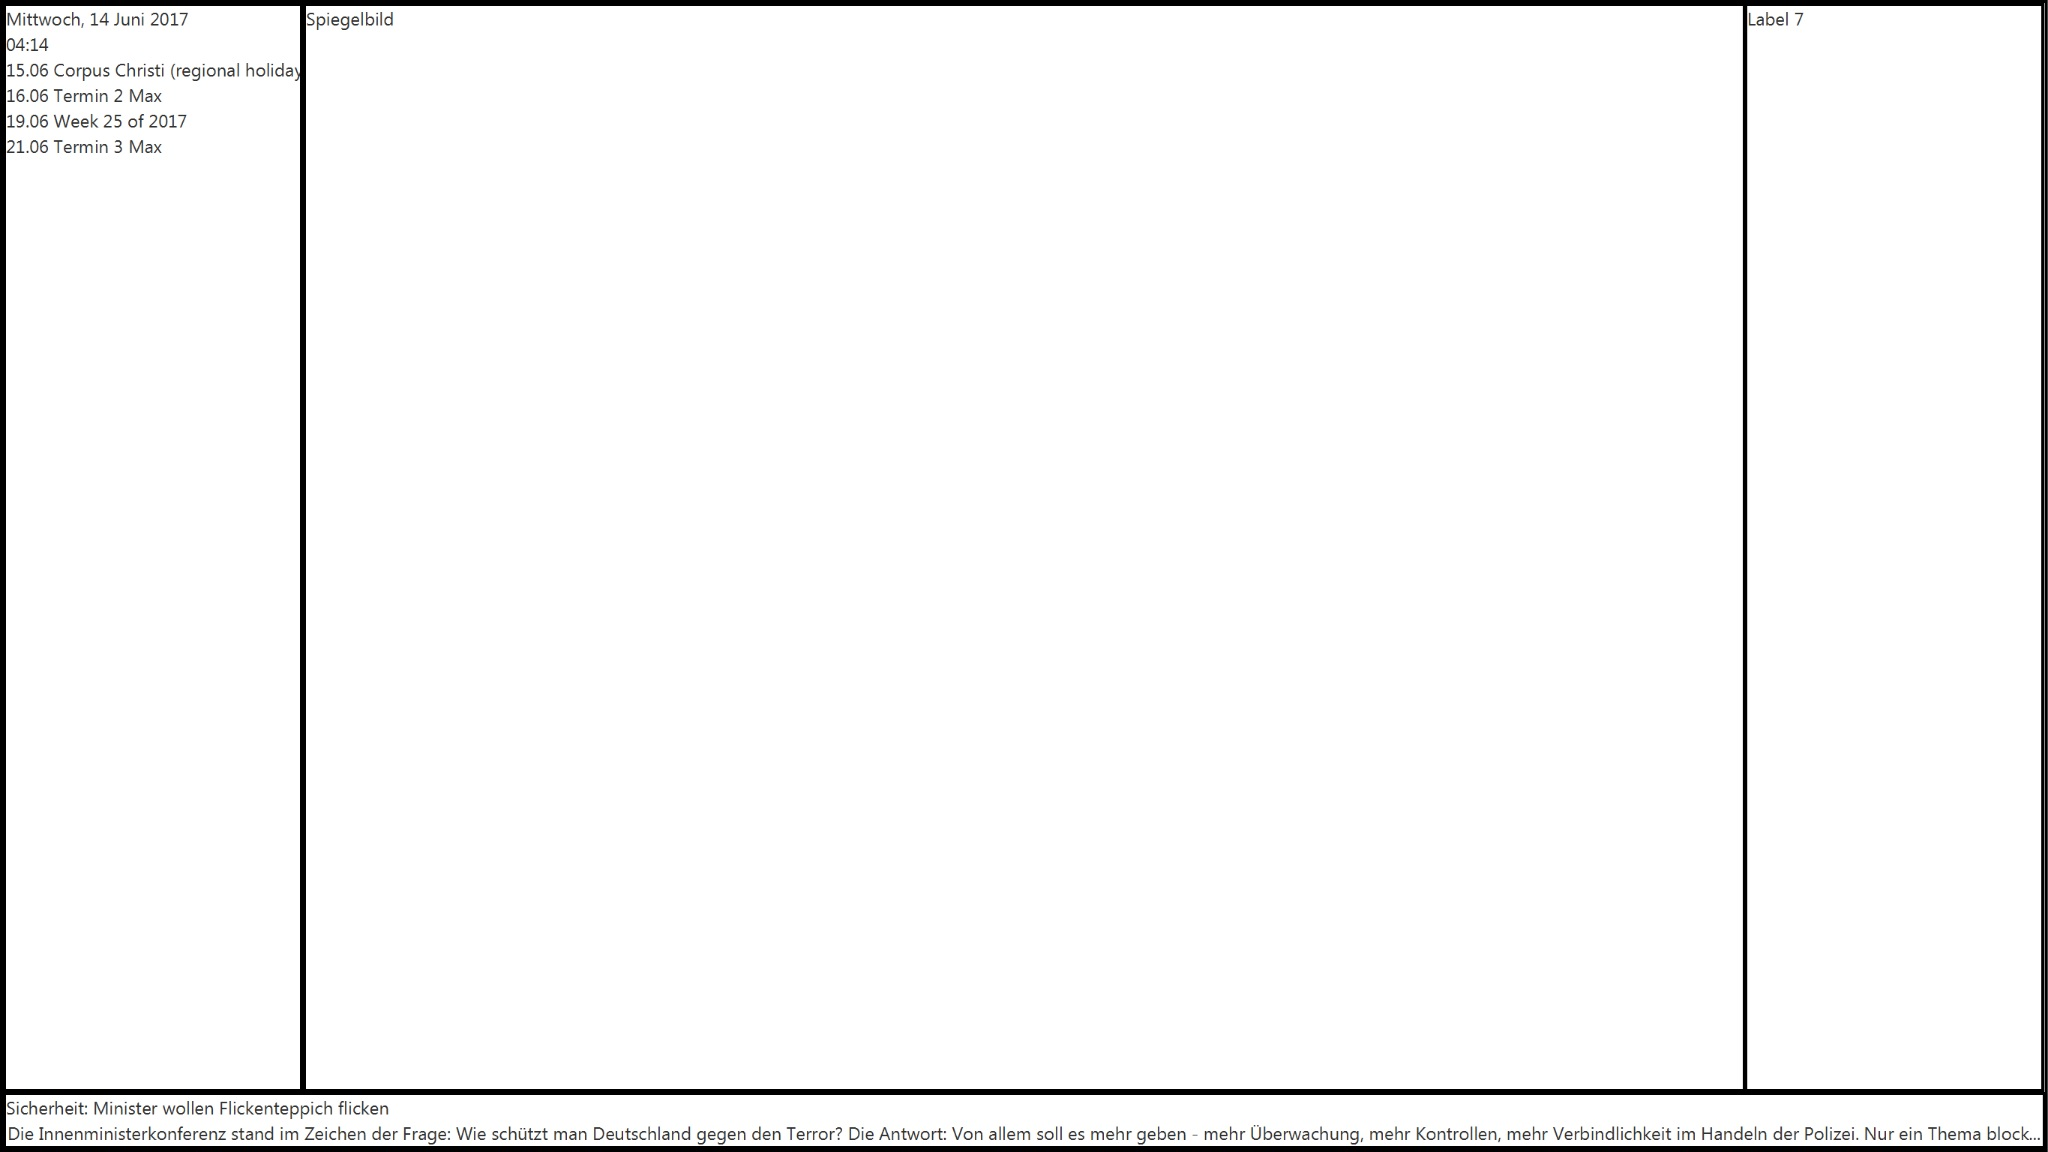
\includegraphics[width=1\textwidth]{figures/magic_mirror_ui_milestone_3.jpg}
	\caption{Bisheriger Stand der UI}
	\label{img:mirror_ui}
\end{figure}

\begin{figure}
	\centering
	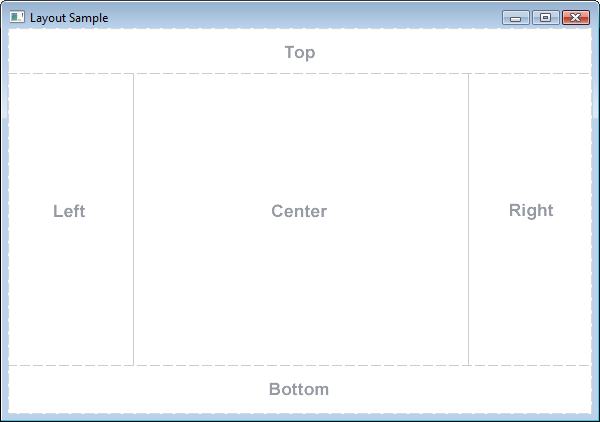
\includegraphics[width=1\textwidth]{figures/magic_mirror_JavaFx_borderpane.png}
	\caption{BorderPane aus JavaFx}
	\label{img:mirror_borderpane}
	\addloflink{https://docs.oracle.com/javase/8/javafx/api/javafx/scene/layout/BorderPane.html}
\end{figure}

\begin{lstlisting}[float=htb,caption={FXMLBspController Klasse - Definiert das Layout auf dem Spiegel und nutzt alle Service-Klassen um die relevanten Informationen abzurufen},label=code:display]
	public void setDateAndTimeLabel() {
		DateFormat formatter = new SimpleDateFormat("EEEE, dd MMMM yyyy");
		String dateString = formatter.format(new Date());
		label1.setText(dateString);
		
		DateFormat timeFormatter = new SimpleDateFormat("hh:mm");
		String timeString = timeFormatter.format(new Date());
		label2.setText(timeString);
	}
	
	public void setCalendarLabel(){
		StringBuilder calendarString = new StringBuilder();
		if(CollectionUtils.isNotEmpty(calendarData)){
			for (Event event : calendarData) {
				DateFormat formatter = new SimpleDateFormat("dd.MM hh:mm");
				DateTime start = event.getStart().getDateTime();
				
				if (event.getStart().getDateTime() == null) {
					start = event.getStart().getDate();
					formatter = new SimpleDateFormat("dd.MM");
				}
				Date date = new Date(start.getValue());
				
				calendarString.append(formatter.format(date) +  " " + event.getSummary() + " " + System.getProperty("line.separator"));
			}
		}else{
			calendarString.append("Keine anstehenden Termine");
		}
		label3.setText(calendarString.toString());
	}
	
	public void setRssFeedLabel(){
		RssFeedService rssFeedService =  new RssFeedService();
		feedMessage = rssFeedService.getFeedData();
		
		label4.setText(feedMessage.getTitle());
		label5.setText(feedMessage.getDescription());
	}
}
\end{lstlisting}






%The following is just a further quick link list compiled to help in creating good scientific presentations.
%\begin{itemize}
%\item \url{http://www.the-scientist.com/?articles.view/articleNo/28818/title/Pimp-your-PowerPoint/}
%\item \url{http://www.northwestern.edu/climb/resources/oral-communication-skills/creating-a-presentation.html}
%\item \url{http://www.nextscientist.com/improve-presentation-skills-of-phd-students/}
%\end{itemize}
